\documentclass[border=3pt]{standalone}
% Preâmbulo compartilhado pelos diagramas TikZ da aula 9 de IHC (Princípios e Diretrizes)
\usepackage[T1]{fontenc}
\usepackage[utf8]{inputenc}
\usepackage{lmodern}
\usepackage{amsmath}
\usepackage{xcolor}
\usepackage{tikz}
\usetikzlibrary{arrows.meta,angles,quotes,decorations.pathmorphing,decorations.pathreplacing,calc,
                positioning,shapes.geometric,shapes.misc,backgrounds,fit,
                math}

% Paleta (mesma dos SVGs originais)
% Paleta da disciplina de IHC: acento roxo (#755099), da capa do livro.
% (o nome "dblue" é mantido para não alterar todos os diagramas)
\definecolor{dblue}{HTML}{755099}
\definecolor{dorange}{HTML}{B3541E}
\definecolor{dgreen}{HTML}{4A7C59}
\definecolor{dred}{HTML}{9C4B4B}
\definecolor{dcream}{HTML}{F4F1EA}
\definecolor{dshade}{HTML}{DDD7C9}

% Função gaussiana (não normalizada por padrão de escala visual)
\pgfmathdeclarefunction{gauss}{3}{%
  \pgfmathparse{1/(#3*sqrt(2*pi))*exp(-((#1-#2)^2)/(2*#3^2))}%
}

% Estilos comuns (prefixo d... para não colidir com chaves internas do pgf)
\tikzset{
  >={Stealth[length=2mm]},
  dguide/.style={gray!55, dashed, line width=0.4pt},
  daxis/.style={gray!60, line width=0.7pt, ->},
  dbody/.style={fill=black!3, draw=black!80, line width=1pt},
  dacc/.style={draw=dblue, line width=1pt},
  dlbl/.style={black!55, font=\small},
  dsub/.style={black!45, font=\footnotesize},
  dstate/.style={circle, draw=black!80, fill=dcream, line width=1pt,
                 minimum size=17mm, font=\large, inner sep=1pt},
  dobs/.style={circle, draw=black!80, fill=dshade, line width=1pt,
               minimum size=14mm, font=\large, inner sep=1pt},
  dbox/.style={rounded corners=2pt, draw=black!80, fill=dcream, line width=1pt,
               align=center, inner sep=6pt},
  dop/.style={circle, draw=black!80, fill=white, line width=1pt,
              minimum size=6mm, inner sep=0pt, font=\small},
  dtrans/.style={->, dblue, line width=1pt},
  dmeas/.style={->, dorange, line width=1pt},
  dcurve/.style={line width=1pt, dblue},
  dcurveb/.style={line width=1.4pt, dorange},
}

\begin{document}
\hyphenpenalty=10000 \exhyphenpenalty=10000 \tolerance=9999 \emergencystretch=3em
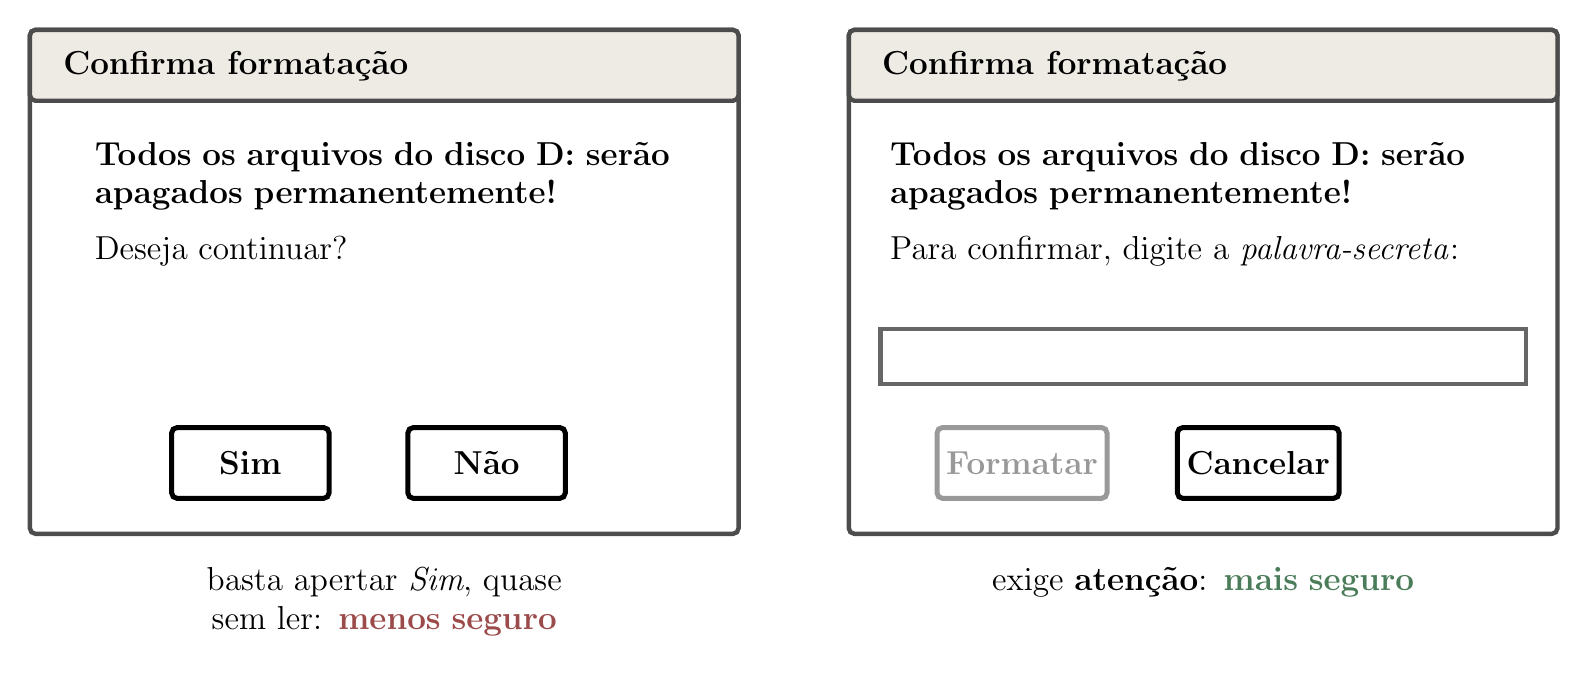
\begin{tikzpicture}[x=1cm,y=1cm]
\tikzset{d/.style={draw=black!70, line width=1.6pt, fill=white, rounded corners=2pt},
        b/.style={draw=black, line width=1.8pt, fill=white, rounded corners=2pt, minimum width=2.0cm, minimum height=0.9cm, font=\large\bfseries}}
\draw[d] (0,0) rectangle (9,6.4); \draw[d, fill=dshade!50] (0,5.5) rectangle (9,6.4);
\node[font=\large\bfseries, anchor=west] at (0.3,5.95) {Confirma formatação};
\node[font=\large, text width=7.6cm, align=left, anchor=north west] at (0.7,5.1) {\textbf{Todos os arquivos do disco D: serão apagados permanentemente!}\\[6pt] Deseja continuar?};
\node[b] at (2.8,0.9) {Sim}; \node[b] at (5.8,0.9) {Não};
\node[font=\large, anchor=north, text width=8.6cm, align=center] at (4.5,-0.3) {basta apertar \emph{Sim}, quase sem ler: \textbf{\textcolor{dred}{menos seguro}}};
\draw[d] (10.4,0) rectangle (19.4,6.4); \draw[d, fill=dshade!50] (10.4,5.5) rectangle (19.4,6.4);
\node[font=\large\bfseries, anchor=west] at (10.7,5.95) {Confirma formatação};
\node[font=\large, text width=8.0cm, align=left, anchor=north west] at (10.8,5.1) {\textbf{Todos os arquivos do disco D: serão apagados permanentemente!}\\[6pt] Para confirmar, digite a \emph{palavra-secreta}:};
\draw[line width=1.6pt, draw=black!60] (10.8,1.9) rectangle (19.0,2.6);
\node[b, text=black!40, draw=black!40] at (12.6,0.9) {Formatar}; \node[b] at (15.6,0.9) {Cancelar};
\node[font=\large, anchor=north, text width=8.6cm, align=center] at (14.9,-0.3) {exige \textbf{atenção}: \textbf{\textcolor{dgreen}{mais seguro}}};
\end{tikzpicture}
\end{document}
